\documentclass{article}
\usepackage[top=10mm, bottom=10mm]{geometry}
\usepackage{amsmath}
\usepackage{graphicx}
\usepackage{circuitikz}
\usepackage{float}

\let\vec\mathbf
\newcommand{\myvec}[1]{\ensuremath{\begin{pmatrix}#1\end{pmatrix}}}

\title{\textbf{Hardware Assignment - Report}}
\author{AI25BTECH11021 - Abhiram Reddy N
 \hspace{0.5cm}   AI25BTECH11008 - Harshith Chiruvella}
 \date{}

 \begin{document}
\maketitle
\section*{Aim and Intro}
The Aim of this project is to display the temperature on LCD . This report details the process of determining the voltage across a PT-100 RTD (Resistance Temperature Detector) as a function of temperature. The least squares method was used to estimate the parameters.

\section*{Instruments,Collecting Data}

\subsection*{Instuments}

Instruments used in this project are :

\begin{itemize}
    \item PT-100 Resistance Temperature Detector
    \item Potentiometer
    \item Arduino Uno and USB Cable
    \item 100~$\Omega$ resistor
    \item Breadboard
    \item Jumper Wires
\end{itemize}

We also made use of the following items for taking the readings

\begin{itemize}
    \item Electric kettle
    \item Digital Thermometer
\end{itemize}

\subsection*{Collecting Data}

The 100~$\Omega$ resistor and the PT-100 were connected in series between the 5~V output pin and the ground pin of the Arduino to create a voltage divider. The other pin of the PT-100 is connected to the A0 pin of the Arduino to measure the voltage across the PT-100.

\begin{center}
\begin{circuitikz}
    \draw
    (0,3) to[battery1, l_=5\,V] (0,0) % reversed polarity: now + is at bottom
    (0,3) -- (3,3)
    to[R, l=100\,$\Omega$] (3,0)
    to[R, l=$P\,\Omega$ (PT-100)] (0,0)
    (3,3) to[short, -*] (4,3)
    node[right]{A0 (Arduino)}
    (3,0) to[short, -*] (4,0)
    node[right]{GND (Arduino)};
\end{circuitikz}
\end{center}


The PT-100 was immersed in an electric kettle filled with water, and a digital thermometer was used to measure the temperature. The C++ code used to drive the Arduino can be found in the appendix.

The kettle was turned on for some time, and then turned off. Once the reading of the digital thermometer became stable, a reading was taken, and the temperature was increased again. A total of 25 readings were taken over a range of temperatures from 27~$^\circ$C to 93~$^\circ$C.

Another 15 readings points were taken to form the validation set. The 25 points were put in the testing set.

\section*{Codes}
The final output code for the Arduino is Arduino.cpp in the codes folder.

\vspace{0.3cm}

And the python codes for the three plots used are also in the codes folder.

\vspace{0.3cm}

And the Training and validation data is in the .txt in codes folder and data folder.

\vspace{0.3cm}

equations.py will output the two main equations.

\vspace{0.3cm}


\section*{Training Data}

This data contains 25 data points which are taken with a thermometer and a kettle and these are plotted in this plot.

\vspace{1cm}

This below plot depicts the training data

\vspace{1cm}

\begin{figure}[H]
    \centering
    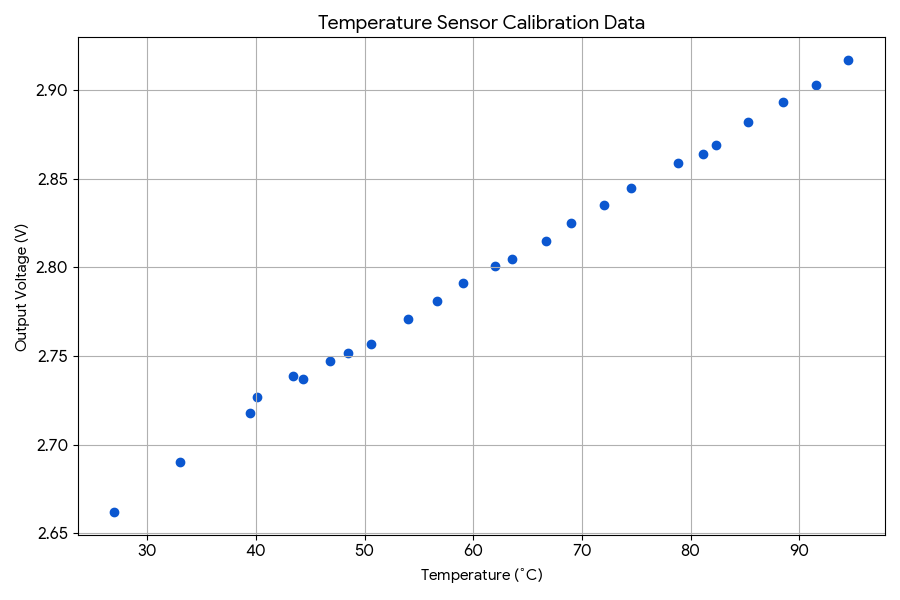
\includegraphics[width=1\textwidth,height=13cm]{figs/training.png}
    \caption{Training Data Plot}
    \label{fig:circuit}
\end{figure}



\section*{Model and Procedure}

We use the quadratic equation to model the voltage across the PT-100 as a quadratic function of temperature.

\begin{figure}[H]
    \centering
    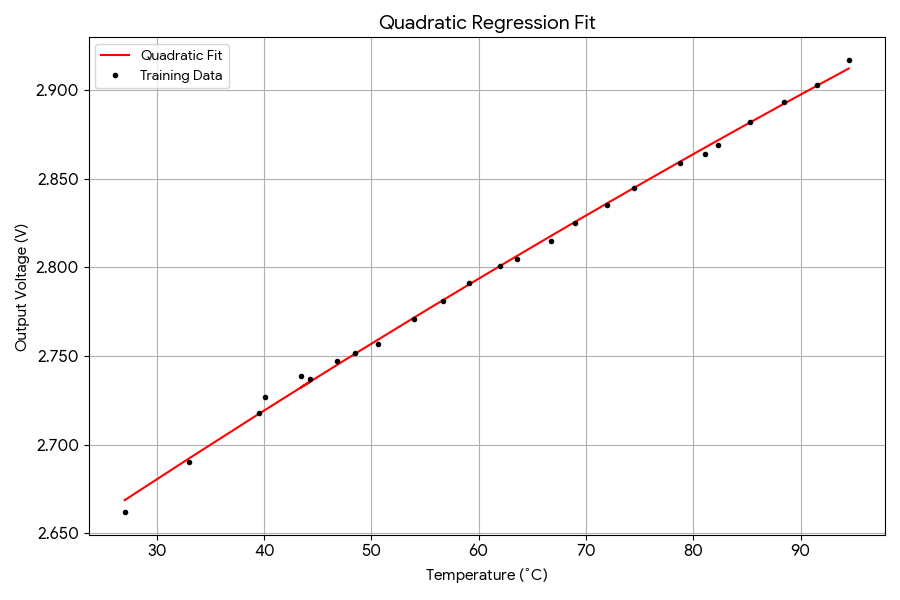
\includegraphics[width=1\textwidth]{figs/model.png}
    \caption{MODEL Plot}
    \label{fig:circuit}
\end{figure}

\subsection*{Equation}

\begin{equation}
V(T) = V(0)(1 + AT + BT^2)
\end{equation}

We can express this as
\[
c = n^\top x
\]
where
\[
c = V(T), \quad n = V(0)
\begin{pmatrix}
1 \\ A \\ B
\end{pmatrix},
\quad
x =
\begin{pmatrix}
1 \\ T \\ T^2
\end{pmatrix}.
\]

We can write the equation in matrix form as
\[
X^\top n = C
\]
where
\[
X =
\begin{pmatrix}
1 & 1 & \cdots & 1 \\
T_1 & T_2 & \cdots & T_n \\
T_1^2 & T_2^2 & \cdots & T_n^2
\end{pmatrix},
\quad
C =
\begin{pmatrix}
V(T_1) \\ V(T_2) \\ \vdots \\ V(T_n)
\end{pmatrix}.
\]
\subsection*{Least Squares Method}

In the least squares method, we try to minimize the squared loss function
\[
L(n) = \| X^\top n - y \|^2
\]
where $y$ is the vector of voltage readings. This can be done by finding the point at which the gradient of the loss function is zero:
\[
\frac{dL(n)}{dn} = 0
\]
The solution which minimizes the loss function is given by
\[
n = (X^\top X)^{-1} X^\top y
\]

The solution may also be calculated using singular value decomposition (SVD). This method reduces rounding errors caused by small numbers, and also handles underdetermined systems better.

In singular value decomposition, we write $X$ in terms of three matrices — two orthogonal matrices $U$ and $V$, and a diagonal matrix $\Sigma$:
\[
X = U \Sigma V^\top
\]
We can then write
\[
n = V \Sigma^{\dagger} U^\top y
\]

The Python program  computes the value of $n$ using the least squares method and also plots the voltage as a function of temperature.

\[
n =
\begin{pmatrix}
2.558197 \\
4.234 \times 10^{-3} \\
-5.1617 \times 10^{-5}
\end{pmatrix}
\]

The approximate model is given by
\[
V(T) = 2.558197 + (4.234 \times 10^{-3})T + (-5.1617 \times 10^{-5})T^2
\]

\vspace{1 cm}
And also we can a function on T in terms of V as

\[
T(V) = 203.0256+ (-379.3723)V + (117.4686)V^2
\]


\section*{Validation}

The model can be validated by using the validation data set.And we can clearly see that the validation data is matching with the model.

\begin{figure}[H]
    \centering
    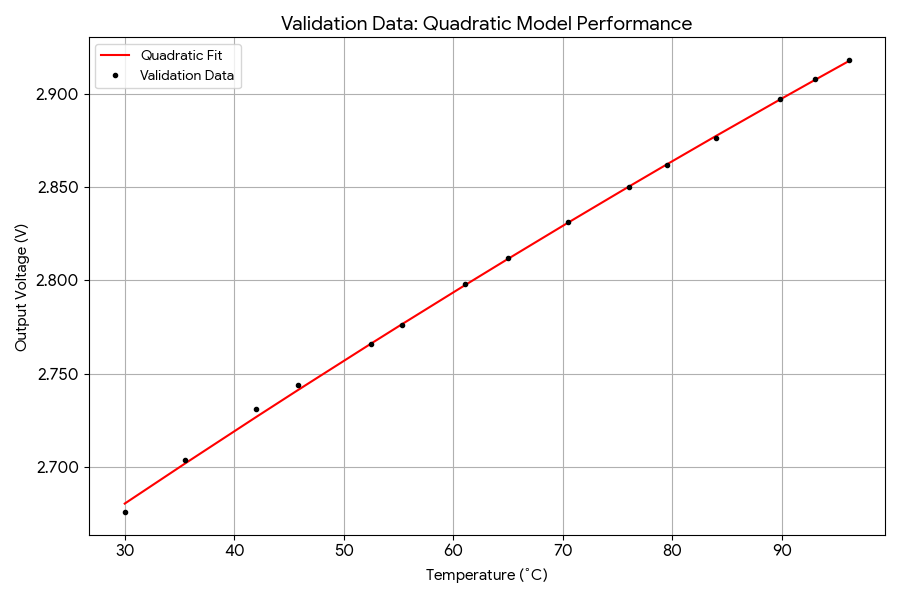
\includegraphics[width=1\textwidth]{figs/validation.png}
    \caption{Validation Plot}
    \label{fig:circuit}
\end{figure}

\section*{Circuit Diagram}

I made this circuit diagram using TinkerCad.

As it does not contain the PT-100 I used multimeter and named it as PT-100. I hope you understand and also the wiring are as exact of my model.

\begin{figure}[H]
    \centering
    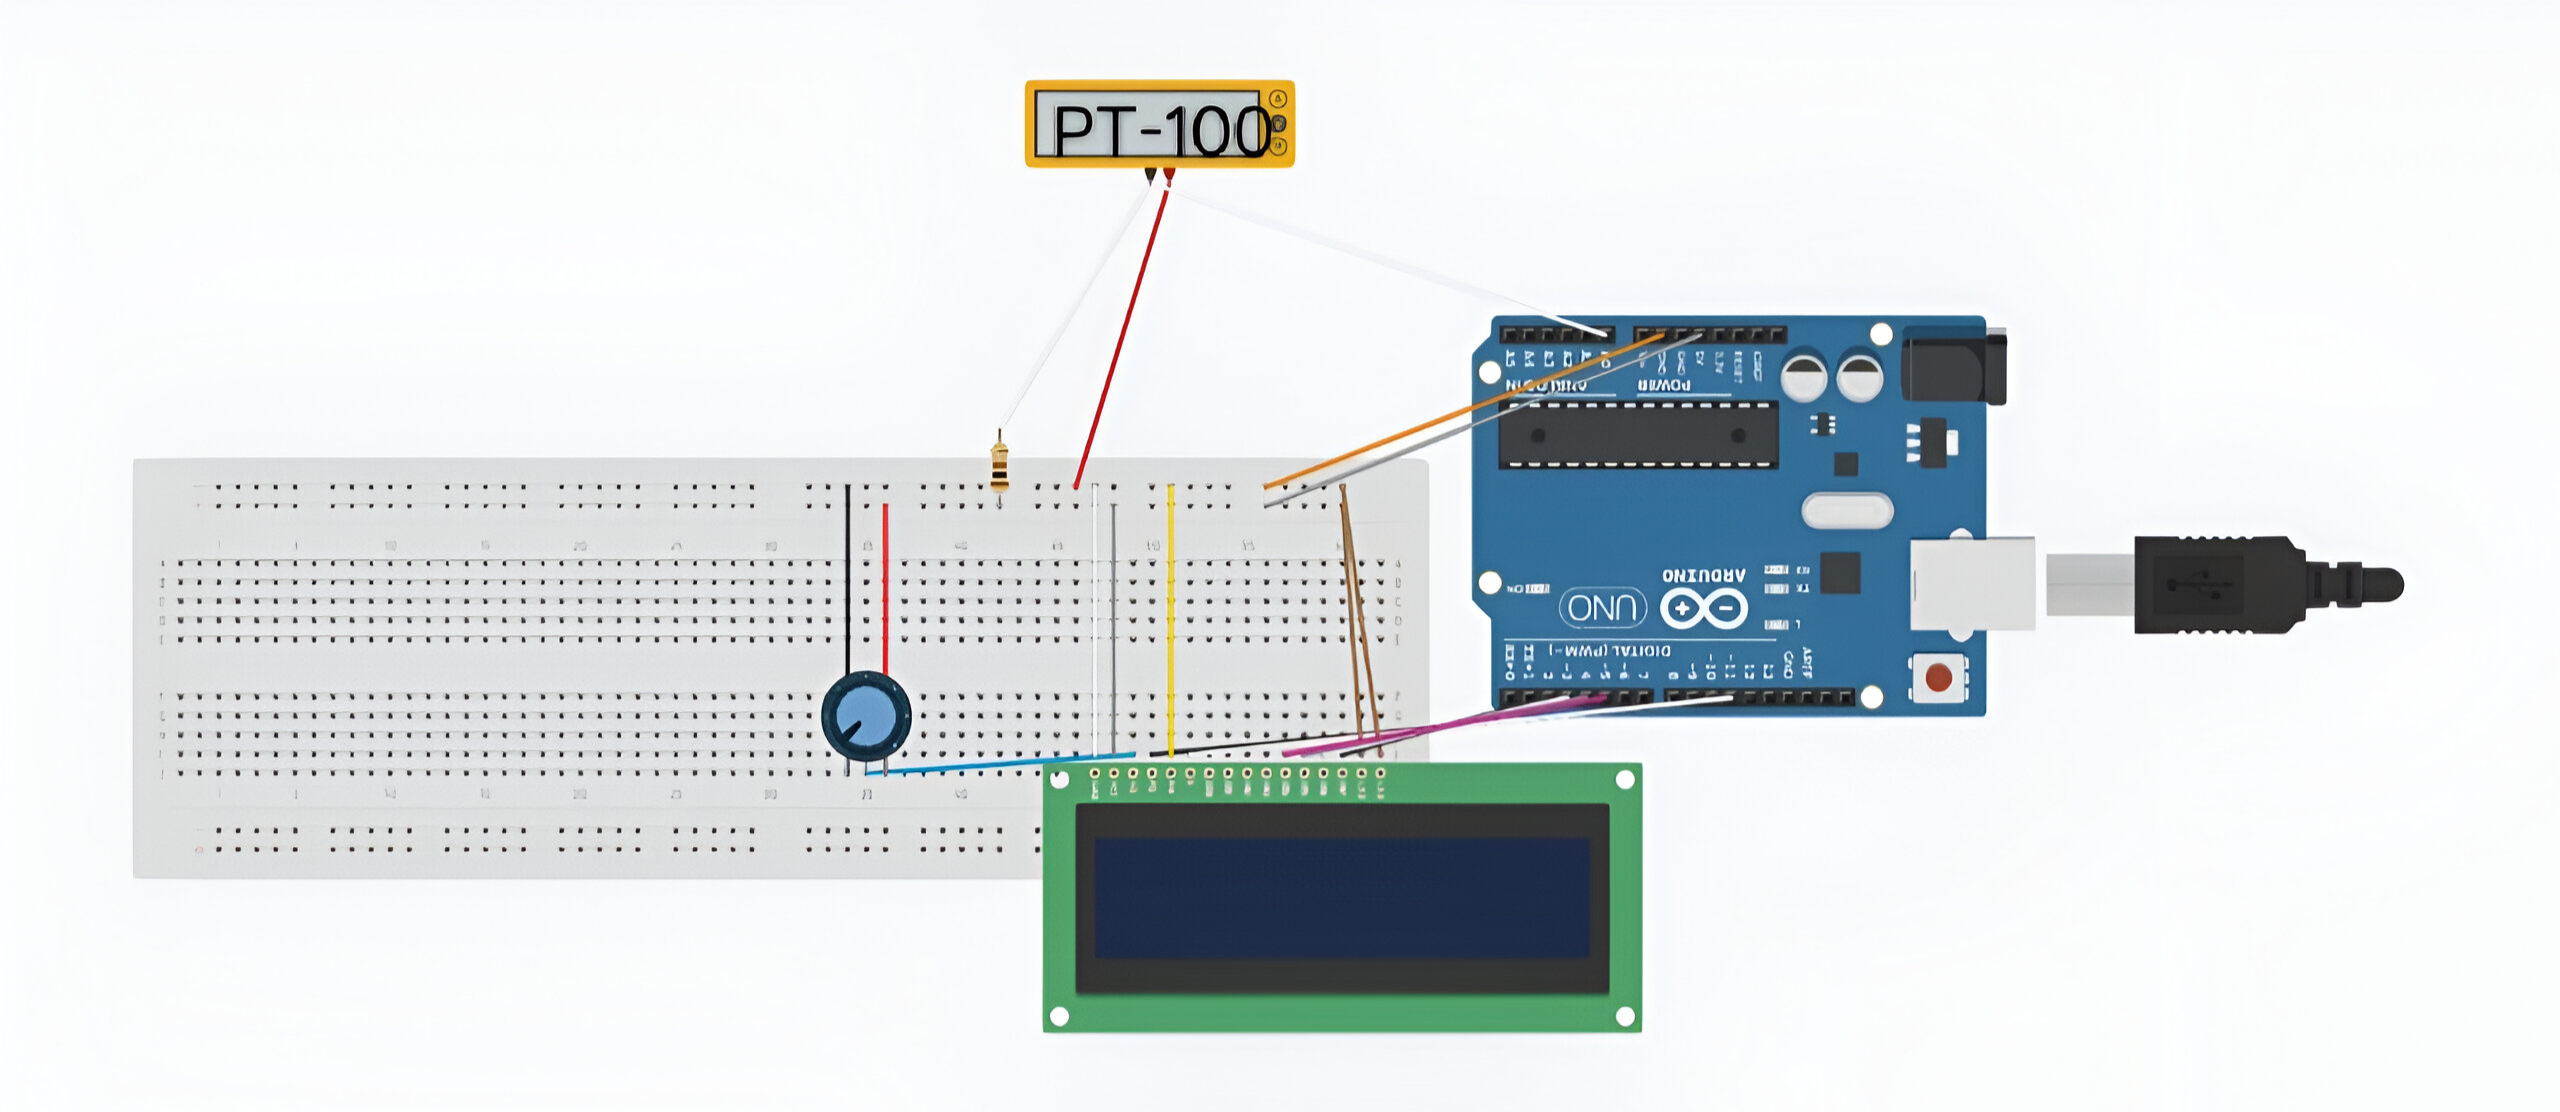
\includegraphics[width=1\textwidth,height=8cm]{figs/Circuit.png}
    \caption{Validation Plot}
    \label{fig:circuit}
\end{figure}


\section*{Error Analysis}

The quadratic calibration model provides a \textbf{very good overall fit} for the training data, as the data points lie closely along the regression curve.

However, a basic analysis of the residuals (the errors between the observed and predicted temperatures) reveals a \textbf{non-random, systematic pattern}:

\begin{itemize}
    \item The error is close to zero at the lowest and highest parts of the temperature range.
    \item The error peaks significantly in the \textbf{negative direction} (model under-predicts the true temperature) in the middle of the range (around $2.74\text{ V}$), with a maximum deviation of nearly $\mathbf{2.0^\circ\text{C}}$.
\end{itemize}

This clear curved pattern in the residuals suggests that the quadratic model does not perfectly capture the sensor's response across the entire range. Using a \textbf{third-order polynomial (cubic fit)} would likely linearize the residuals, resulting in a lower maximum error and a more accurate calibration curve overall.


\end{document}